% Tutorial 06

\subsection{Tutorial 6: NN(QM)/MM simulations with the BuRNN approach}
The Buffer Region Neural Network (BuRNN) approach \cite{Lier2022BuRNN} is a hybrid quantum mechanics/molecular mechanics (QM/MM) \cite{Warshel1976QM/MM, Senn2009QM/MM} simulation method. The system is therefore partitioned into regions having different levels of theory, a QM and a classical MM region. 

In-between the two regions an additional buffer region is introduced to be treated at both levels of theory (Figure~\ref{BuRNN_scheme}, a). The interactions between the QM region (inner region) and the buffer are described by an atomistic neural networks (NN). 

The total potential energy of the system is calculated as follows:

\begin{equation}
  \begin{aligned}
  V_{tot} = V^{QM}_{\mathbb{I+B}} - V^{QM}_{\mathbb{B}} + V^{MM}_{\mathbb{B}} + V^{MM}_{\mathbb{O}}
    \end{aligned}
\end{equation}

 The energy difference of the first two terms is directly described by a neural network potential: 
 
\begin{equation}
  \begin{aligned}
  V_{tot} \cong \mathrm{V}_{\mathbb{I+}\Delta\mathbb{B}}^{NN} + \mathrm{V}_{\mathbb{B+O}}^{MM}
    \end{aligned}
\end{equation}

 As a NN model we use SchNet \cite{Schuett2017SchNet, Schuett2018SchNet,Schuett2019SPK}, a deep learning architecture implemented in the MD engine of GROMOS.
 
In this tutorial we will prepare training data and NN models for methanol and finally run BuRNN simulations based on the trained models.

\begin{figure}[H]
\centering
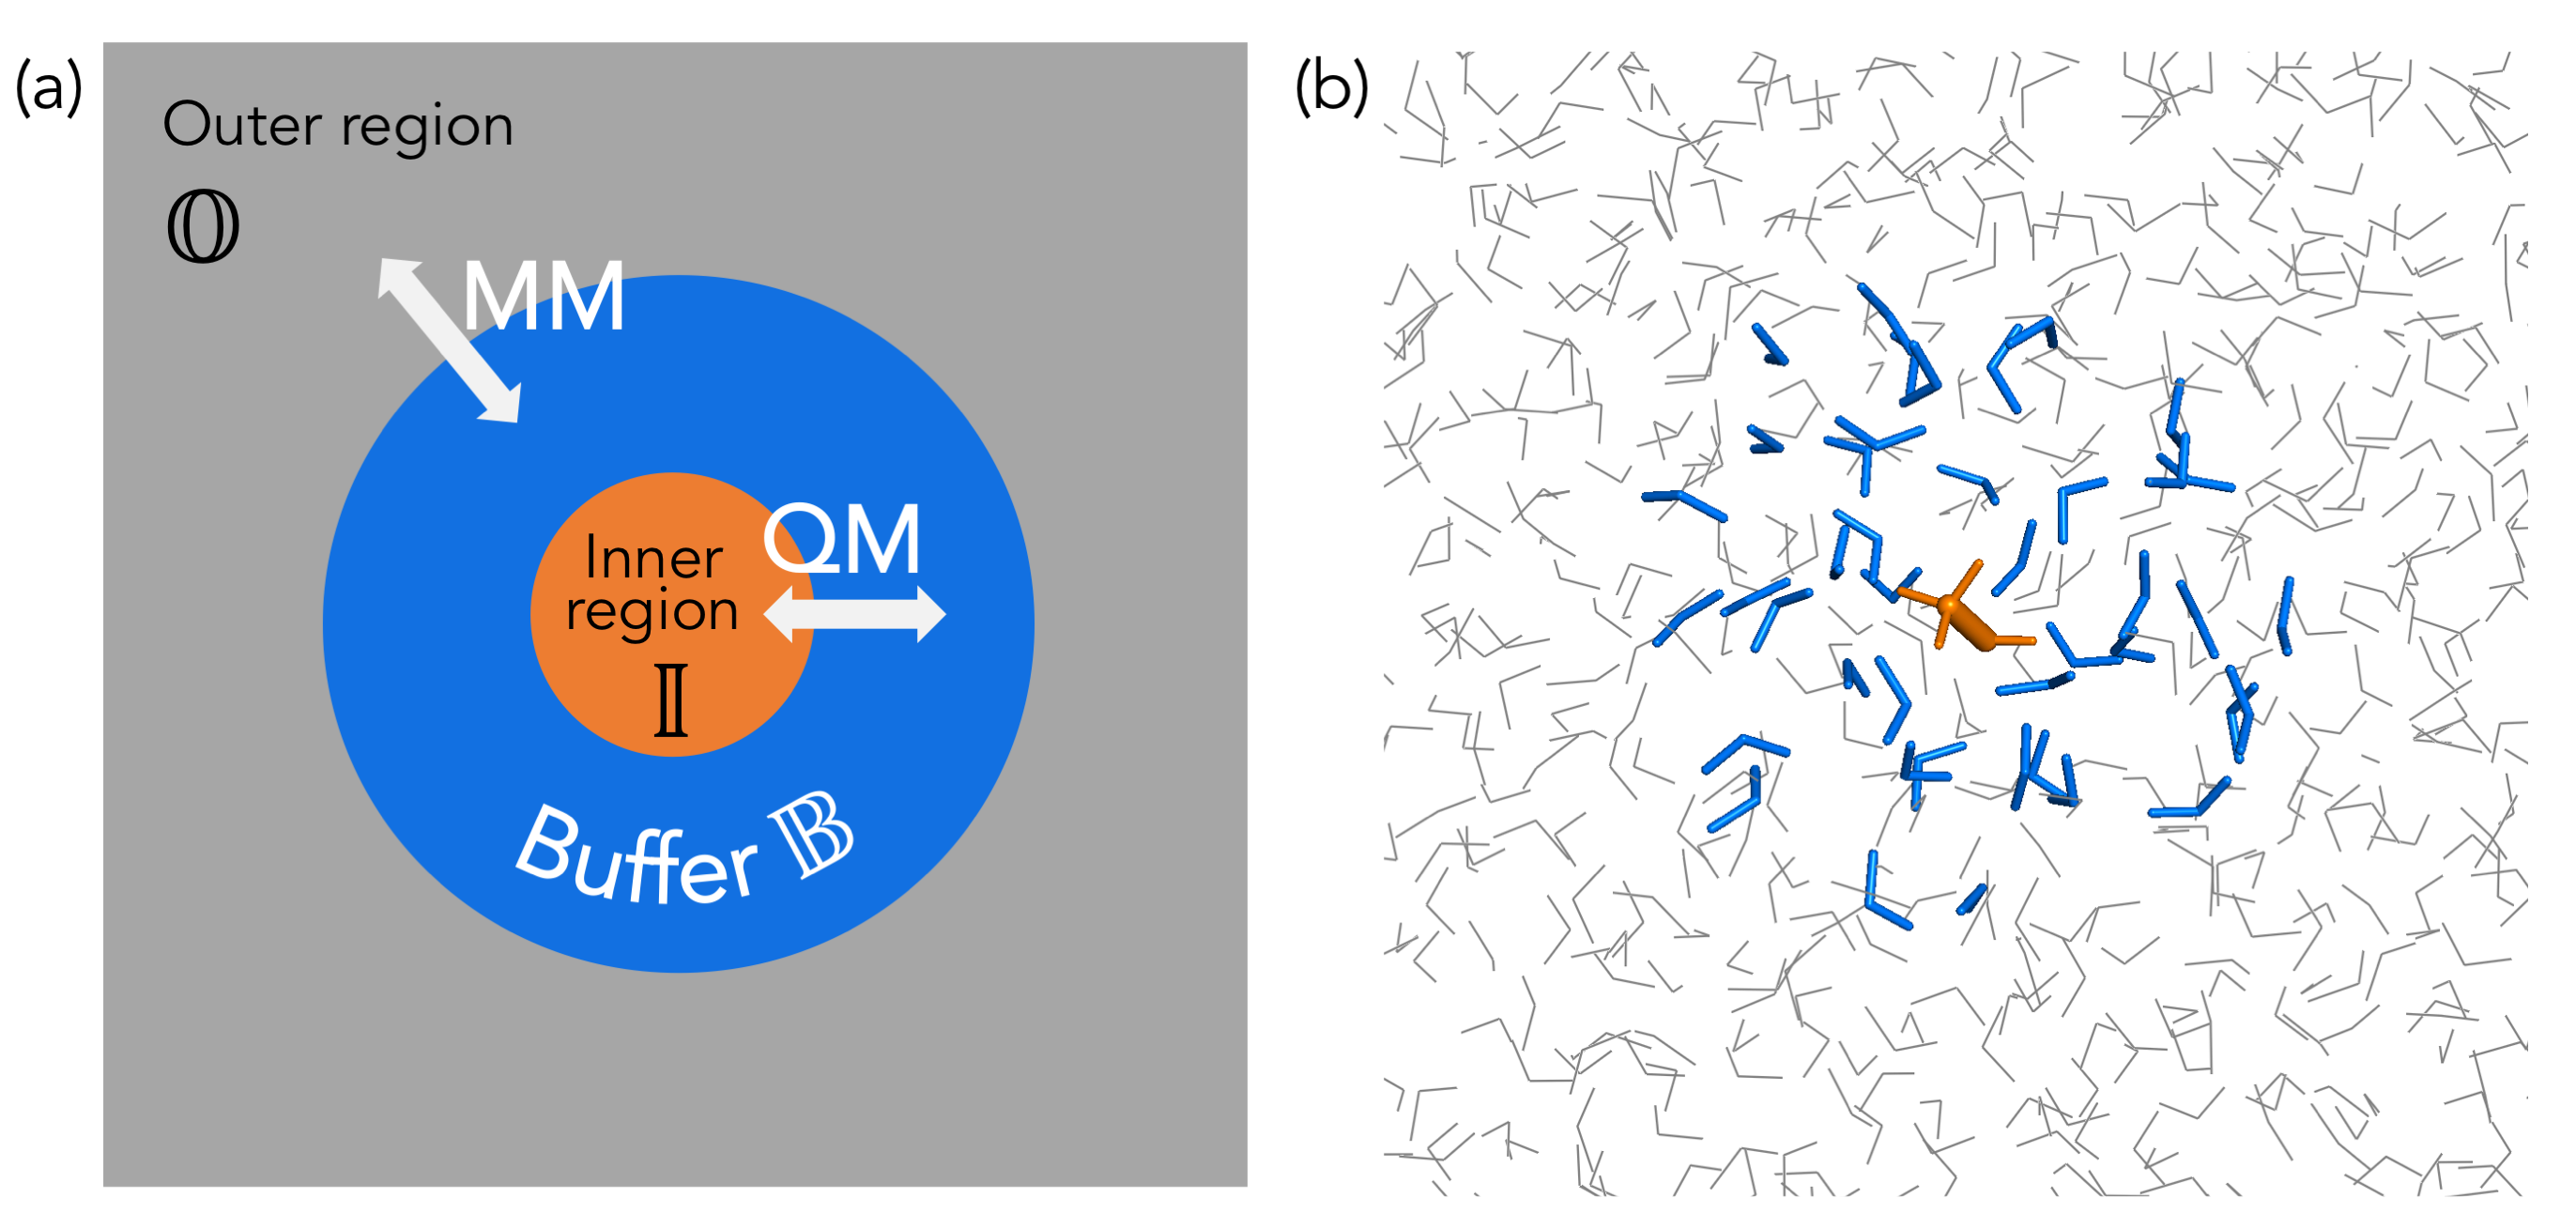
\includegraphics[scale=.33]{../09_tutorial_06/figures/BuRNN_scheme}
\caption{(a) BuRNN scheme with its three regions: Inner region (orange) described by quantum mechanics (QM), buffer region (blue) described by QM and classical molecular mechanics (MM), outer region (grey) described by MM. (b) Test system: methanol solvated in SPC water. Methanol therefore builds the inner region, two shells of water will be the buffer region, the rest of the water box serves as outer region.}
\label{BuRNN_scheme}
\end{figure}


\subsubsection{Installation}
\paragraph{Prerequisites}
To compile and install GROMOS with the interface to SchNetPack (spk) to run NN models, you first need to have installed SchNetPack and the pybind11 library. The interface uses the pybind11 library to call the model evaluation functions in the Python code of SchNetPack. To install the SchNetPack and pybind11 library on your system, please follow their installation. Tested version of SchNetPack is 1.0.0 and pybind11 is 2.6.2.

\paragraph{GPU acceleration}
This part is optional to improve the efficiency of the simulations. The tasks in this tutorial are small enough to be run CPU-only in reasonable time. For the production runs this is inefficient since the training and evaluation of models on a GPU is usually many-folds faster. NN/MM MD simulations in GROMOS profit from this as well. Unfortunately, setting up your system to support the GPU acceleration is strongly architecture specific and is dependent on the installed CUDA and Pytorch versions. Please follow the installation instructions of CUDA and Pytorch to run tasks with the GPU acceleration.

\paragraph{GROMOS compilation}
Compilation of the NN-enabled version of GROMOS is activated by the \texttt{--enable-schnetpack} flag in the configuration step. The \texttt{configure} script looks up the pybind11 library automatically; however, based on the versions of the packages and the architecture, it might not be found. In that case you should provide the flags \texttt{PYFLAGS} and \texttt{PYLDFLAGS} to the \texttt{configure} script. The \texttt{PYFLAGS} variable holds the C preprocessor flags, which can be obtained by calling

\begin{lstlisting}[breaklines=true, breakatwhitespace=false]
python3 -m pybind11 --includes
\end{lstlisting}

The \texttt{PYLDFLAGS} are the linker flags. Depending on the Python version, they can be generated by calling either 

\begin{lstlisting}[breaklines=true, breakatwhitespace=false]
python3-config --ldflags
\end{lstlisting}

for Python<3.8, or 

\begin{lstlisting}[breaklines=true, breakatwhitespace=false]
python3-config --ldflags --embed
\end{lstlisting}

for newer versions. An example of the \texttt{configure} script then could be:
\begin{lstlisting}[breaklines=true, breakatwhitespace=false]
$./configure --enable-schnetpack PYFLAGS='-I/path/to/include/python3.7 -I/path/to/lib/python3.7/site-packages/pybind11/include' PYLDFLAGS='-L/path/to/lib/python3.7/config -L/path/to/lib -lpython3.7 -lcrypt -lpthread -ldl -lutil -lrt -lm'
\end{lstlisting}

Further steps follow the standard compilation:
\begin{lstlisting}[breaklines=true, breakatwhitespace=false]
$ make
$ make install
\end{lstlisting}


\subsubsection{Training dataset generation and model training}
In order to train NN models, QM data points for building a database have to be generated first. We decided to use semi-empirical QM calculations to present the BuRNN approach in this tutorial, as it takes least computational resources. We will run in it with the MOPAC \cite{Stewart1990MOPAC, Stewart2013MOPAC} program. Usually the user decides which reference method will be used, depending on the system and the accuracy requirements.

This chapter will be accompanied by the \texttt{meoh.ipynb} jupyter notebook for sake of simplicity. It will use the in-house written python modules \texttt{gromos} for editing GROMOS files, \texttt{mopac} to run QM calculations in MOPAC and \texttt{additional\_spk\_utils} for i.e. building the training database.

\paragraph{Generating QM and Buffer region}
In the first step classical MD simulations of the system are run as described in tutorial 1. Explicit hydrogen atoms need to be added for subsequent QM calculations. The required files for the simulations are provided.
%\texttt{meoh.top}, \texttt{meoh.cnf}, \texttt{em_solute.imd}, \texttt{em_solute.run}, \texttt{sim_box.arg}, \texttt{sim_box.arg}, \texttt{em_solvent.imd}, \texttt{em_solvent.run},...  
Then the QM zone (inner + buffer region) from each snapshot is extracted using the GROMOS++ program \texttt{filter}. This program writes out coordinate trajectories for atoms that are within a specified distance of a certain part of the system. For methanol we specify the carbon to be the center (\texttt{@atoms 1:a}) and filter with a chargegroup-based cut-off (\texttt{@pairlist CHARGEGROUP}) of 0.5 (or 0.55) nm radius (\texttt{@cutoff 0.5}). The optimal/reasonable size for the buffer region can be determined from an rdf analysis. It should be as small as possible, as we want to save computational effort for the following QM calculations. The chargegroup cut-off scheme is important as we want to include full water molecules in the QM calculations. We provide an argument file to run filer

\begin{lstlisting}[breaklines=true, breakatwhitespace=false]
$ filter @f filter_meoh.arg > filter_meoh.out
\end{lstlisting}

\paragraph{QM calculations}
In this part we will mainly focus on the concept of QM geometry optimization (GO) and single point calculations (SP) in the context of BuRNN.
Once we have the coordinates of the QM zone, the QM energy minimization (GO) will optimize the atomic positions to find the local minimum of the QM potential energy surface. This calculation will not only find the local energy minimum, but also connects the classical snapshots with the optimal QM conformations and thus represents sufficient part of the conformational space of the system. We will therefore include all steps into the training dataset, but we need to be aware that the training data set will be significantly increased in size. A lot of similar structures will be present in the end of the minimization and therefore clustering before proceeding with the next step would be recommended.

For each (remaining) energy minimization steps, a single point (SP) QM calculation is required to receive the associated QM energy and forces. The SP calculation is not only done for the whole QM zone (inner + buffer region), but also for the buffer region alone. The coordinates of the buffer region are identical for the two calculations. The number of atoms for the inner region is required, as these atoms need to be deleted for the second calculation (buffer only). Furthermore, the geometry of water molecules in the buffer region need to be preserved as in the following BuRNN simulations the bonds will be constrained by the SHAKE algorithm\cite{RYCKAERT1977SHAKE}.

We will use the MOPAC software and run the QM calculations via the \texttt{mopac} module. Any other QM software can be used and any level of QM theory is possible.

\paragraph{Building a training database}
In this chapter we will explain how to build the ASE (atomic simulation environment) \cite{Larsen2017ASE} database from the previously calculated energies and forces of the snapshots. 

We will use the \texttt{additional\_spk\_utils} module for storing the relevant properties and metadata in the database. The absolute energies of the complex (inner + buffer region) and buffer, the energy differences between the two and the differences between the forces. Additionally we store reference energies (energies in vacuum) for all components in the QM zone separately. In our example it would be the energy of one methanol molecule in vacuum and of one water molecule in vacuum. 

To calculate the interaction energy between inner region and buffer region, the reference energies are subtracted. Note that the number of water molecules in the buffer region has to be multiplied with the reference energy of one water molecule.


\paragraph{Model training}
The last step before running BuRNN simulations is the NN model training. In the previous parts, the ASE database was created based on structures from QM energy minimizations and SP calculations. We now use SchNetPack for training the models as this NN model is also integrated in the BuRNN simulation engine.  

For the model training we use two scripts, a python \texttt{spk\_run\_standard.py} and a bash \texttt{spk\_run.sh} script. The python script loads the data from the previously prepared ASE database and splits it into training, validation and test set (we will use 80, 10, 10\% of the dataset). After preparing the data, the model can be built and trained in three steps: defining the input modules, building a model representation and defining an output module.

Many parameters have to be set; we use the bash script to call the python 
\texttt{spk\_run} script and define the paths and all the relevant (hyper)parameters.
Following parameters are defined in our example training:
\begin{enumerate}
    \item[-] property = property to be predicted by the model (default 'energy')
    \item[-] derivative = derivative of the property to be predicted (default 'forces')
    \item[-] rho = weigth factor for the property and derivative, respectively (default (0.01, 0.99))
    \item[-] split = determines how many training, validation and test data will be selected, the first value for training data size, the second for validation data size, the rest of the dataset is used for the model evaluation (default (None, None))
    \item[-] batch\_size = batch size (default 8)
    \item[-] device = cpu or cuda (default 'cuda')
    \item[-] n\_epochs = maximum number of training epochs (default 5000)
    \item[-] lr = learning rate (default 0.0001)
    \item[-] lr\_patience = learning rate will be decreased after the certain number of epochs without improvement of the model (default 10)
    \item[-] lr\_min = minimal learning rate, when the value is reached, the training process is stopped (default 1e-06)
    \item[-] cutoff = cutoff for long-range interactions (default 100.0)
    \item[-] num\_gaussians = number of gaussians to describe (default 25)
    \item[-] features = number of atom-wise features (default 128)
    \item[-] interactions = number of interaction blocks (default 3)
\end{enumerate}

As we train on energies and forces, a combined loss function for optimizing the weight parameters will be used that predicts and obtains forces automatically as derivatives of the energies. For that a loss weight (parameter called rho) is introduced to control the trade-off between energy loss and force loss.

It is reasonable to use the default values to start with the training and then optimize them. The number of atom-wise features and the number of interaction blocks are the most important hyperparameters of the SchNet architecture, as they define the model complexity and therefore the precision and computational costs. 

The training will produce several files in the model-path directory. The model, the evaluation file, a training log file, a file with the random split, a checkpoint file and a json file with the model settings. The checkpoint file is written periodically and can be used to restart the training.   

For the BuRNN simulations we provided fully trained models that you can find in the 
\texttt{path/provided\_models} directory.

\paragraph{Model evaluation}
??


\subsubsection{BuRNN simulations}
For a BuRNN simulation, the QM and buffer regions have to be defined. Therefore the QM atoms have to be specified and the buffer region has to be adjusted by setting a cut-off around the QM region. This information together with other specifications will be stored in an additional input file \texttt{meoh.qmm}:

\begin{lstlisting}[breaklines=true, breakatwhitespace=false]
TITLE
qmmm specification file for BuRNN  
END
QMUNIT
# QMULEN    QMUENE    QMUFOR    QMUCHR
     0.1     4.184     41.84       1.0
END
\end{lstlisting}

The \texttt{QMUNIT} block may convert units of the model by a conversion factor for distances (\texttt{QMULEN}), energies (\texttt{QMUENE}), forces (\texttt{QMUFOR}), and charges(\texttt{QMUCHR}).

\begin{lstlisting}[breaklines=true, breakatwhitespace=false]
NNDEVICE
auto
END
NNMODEL
/path/to/best_model
# MT LT
   0  1
END
NNVALID
/path/to/best_model2
# NUMSTP THRSH FCON 
       1   5.0  0.0
END
\end{lstlisting}

Having created the NN models described in the previous chapters, the paths to the models have to be specified and some parameters for the model evaluation. The \texttt{NNDEVICE} block decides if it should be run on cuda (gpu) or cpu. If you specify auto, it will first try to run with cuda, if it is not available switch to cpu. 
In the next block, \texttt{NNMODEL}, the path to the best model is given. The model type is set to 0 which means that BuRNN will be run with a single NN evaluation on the previously trained energy differences. It would also be possible to calculate differences just during the simulation in a combined model or even calculate it with QM on the fly by setting it to 1. The learning type is set to 1 for a standard calculation. 
The \texttt{NNVALID} block is optional and used if a validation model is evaluated to compare the energy differences to the individually trained \texttt{NNMODEL}. In case, we have to set the path to the validation model. The two NNs will be compared at every nth step (\texttt{NUMSTP}), the difference will be deemed accurate if it is below the threshold (\texttt{THRSH}). If it’s above the threshold, the force constant (\texttt{FCON}) can be set positive which pushes back the atoms to a configuration that agrees better with both models. 
We set the threshold to 5 kJ/mol which is above but close to the chemical accuracy of 1 kcal/mol and calculate the difference between the models at every time step. This can be easily changed when we need to generate coordinates that are not included in the training set or when the simulation is not stable yet. When we have a stable simulation, we can e.g. check the differences at about every 100th step.

\begin{lstlisting}[breaklines=true, breakatwhitespace=false]
QMZONE
# CHG MULT
    0    1
# RESIDUE   ATOM     QMI   QMZ   QMLI
   1 MeOH   CA         1     6      0
   1 MeOH   OB         2     8      0
   1 MeOH   HA1        3     1      0
   1 MeOH   HA2        4     1      0
   1 MeOH   HA3        5     1      0
   1 MeOH   HB1        6     1      0
END
BUFFERZONE
# CHG MULT CUT-OFF 
    0    1     0.5
# RESIDUE   ATOM     QMI   QMZ   QMLI
   1 SOLV   OW         7     8     0
   1 SOLV   HW1        8     1     0
   1 SOLV   HW2        9     1     0
   2 SOLV   OW        10     8     0
   2 SOLV   HW1       11     1     0
   2 SOLV   HW2       12     1     0
   ...
END
\end{lstlisting}

These blocks finally contain the atoms that are part of the inner region (\texttt{QMZONE}) and might be part of the buffer (\texttt{BUFFERZONE}). In the first line of both blocks we specify charge and multiplicity of the species, in the \texttt{BUFFERZONE} block we also define the cut-off which we chose to be 0.5 nm. According to the cut-off size, the atoms that are included in the \texttt{BUFFERZONE} block will become buffer atoms as soon as they cross the cut-off during the simulation.

Next to the separate input file, the \texttt{meoh.imd} file requires a \texttt{QMMM} block:
\begin{lstlisting}[breaklines=true, breakatwhitespace=false]
QMMM
# NTQMMM NTQMSW RCUTQM NTWQMMM QMLJ QMCON      
 MMSCALE
       1      5    1.4       0    0     0
    -1.0
END
\end{lstlisting}

Most parameters are only relevant for conventional QM/MM simulations and will therefore not be explained in detail.
Setting the first parameter, \texttt{NTQMMM=1}, QM/MM hybrid simulations are turned on (with mechanical embedding). \texttt{NTQMSW} further determines which software will be used for the QM calculation. If \texttt{NTQMSW=5}, instead of a QM package (1-4), SchNetPack will be called. The cut-off determined by \texttt{RCUTQM} is only relevant for electrostatic or polarizable embedding using QM packages. \texttt{NTWQMMM} can be used if QM/MM related data should be written out every nth step to a separate trajectory. For BuRNN simulations we don’t want to calculate LJ between QM atoms and set distance restraints in the QM zone, therefore \texttt{QMLJ=0} and \texttt{QMCON=0}. With \texttt{MMSCALE} we can scale MM charges (by a scaling factor), but if \texttt{MMSCALE<0} no scaling is applied.

%Provide following files:
%meoh.qmm
%meoh.imd
%mk_script.arg
%mk_script.lib (depending on the environment, activation of libs)

\subsubsection{BuRNN (example) analysis}
The trajectories created from a BuRNN simulation are the same as from plain MD simulations, meaning that we can do any analysis.

Here we decided to show hydrogen bonds that are formed between the methanol treated at the QM level and the MM waters around. It is done as follows:

\begin{lstlisting}
$ hbond @f hbond_meoh.arg
\end{lstlisting}

(further explanation what to do with the hbond output?)

\subsubsection{Advanced options}
\paragraph{Including a charge model}
For running BuRNN simulations with dynamic QM charges, charges first need to be calculated with the QM method of choice and included in the training dataset. A separate NN has to be trained for the charges. SchNet was therefore adapted and the version can be found in this repository: https://github.com/juliawestermayr/schnetpack.
In the \texttt{charge.qmm} file the \texttt{NNCHARGE} block has to be added. 

\begin{lstlisting}[breaklines=true, breakatwhitespace=false]
NNCHARGE
/path/to/best/charge_model
# NUMSTP
       1
END
\end{lstlisting}
This block contains the path to the NN charge model and that the charges should be updated at every nth step (\texttt{NUMSTP}). 

%\paragraph{Adaptive sampling}
